\documentclass{beamer}

\usepackage{listings}
\lstset{ % General setup for the package
    language=VHDL,
    numbers=left,
    frame=tb,
    tabsize=4,
    columns=fixed,
    showstringspaces=false,
    showtabs=false,
    keepspaces,
    commentstyle=\color{brown},
    keywordstyle=\color{blue},
    stringstyle=\color{red},
    title=\lstname,
    basicstyle = \tiny
}

\usecolortheme{beaver}
\setbeamertemplate{navigation symbols}{}

\title{Mandelbrot Pong}
\subtitle{EE-334 Digital systems design}
\author[Thür, Mheni] % (optional, for multiple authors)
	{Simon~Thür \and Lokman~Mheni}
\institute[EPFL]{EPFL SEL-BA5}
\subject{Digital systems design}

\begin{document}
\frame {
    \titlepage
}

\begin{frame}
    \frametitle{Table of Contents}
    \tableofcontents[currentsection]
\end{frame}



\begin{frame}
    \frametitle{Overview}
    Implemented features:
    \begin{itemize}
        \item VGA-Controller
        \item Memory for storing image
        \item Pong game mechanics
        \item Pong sprites
        \item Mandelbrot generator
        \item Mandelbrot zoom animation
    \end{itemize}

\end{frame}


\section{VGA Controller}
\begin{frame}
    \sectionpage
\end{frame}

\begin{frame}
    \frametitle{VGA Controller}
    \begin{itemize}
        \item 2 Counters (x and y)
        \item Front porch, pulse, and backporch at Beginning of frame
        \item Edge detector on Vertical Sync (VSedgexSO corresponds to new frame)
        \item X,Y output corresponds to next color wanted
    \end{itemize}

    \begin{equation}
        \begin{split}
            X_{out} &= X{cntr} - (FP_{HS} + P_{HS} + BP_{HS})+1\\
            Y_{out} &= Y{cntr} - (FP_{VS} + P_{VS} + BP_{VS})
        \end{split}
    \end{equation}
\end{frame}


\section{Memory}
\begin{frame}
    \sectionpage
\end{frame}

\begin{frame}[fragile]
    \frametitle{Memory}
    \framesubtitle{Coordinate mapping}
    \lstinputlisting[firstline=297,lastline=302]{../_00FINAL_PROJECT/src/mandelbrot_top.vhdl}
    firstline=297,lastline=302

\end{frame}



\begin{frame}
    \frametitle{Memory}
    \framesubtitle{Size constraints}
    \begin{alertblock}
        {16 bit constraint on memory address}
        Not enough space for 2 images (without reducing image resolution farther)
    \end{alertblock}
    \begin{figure}
        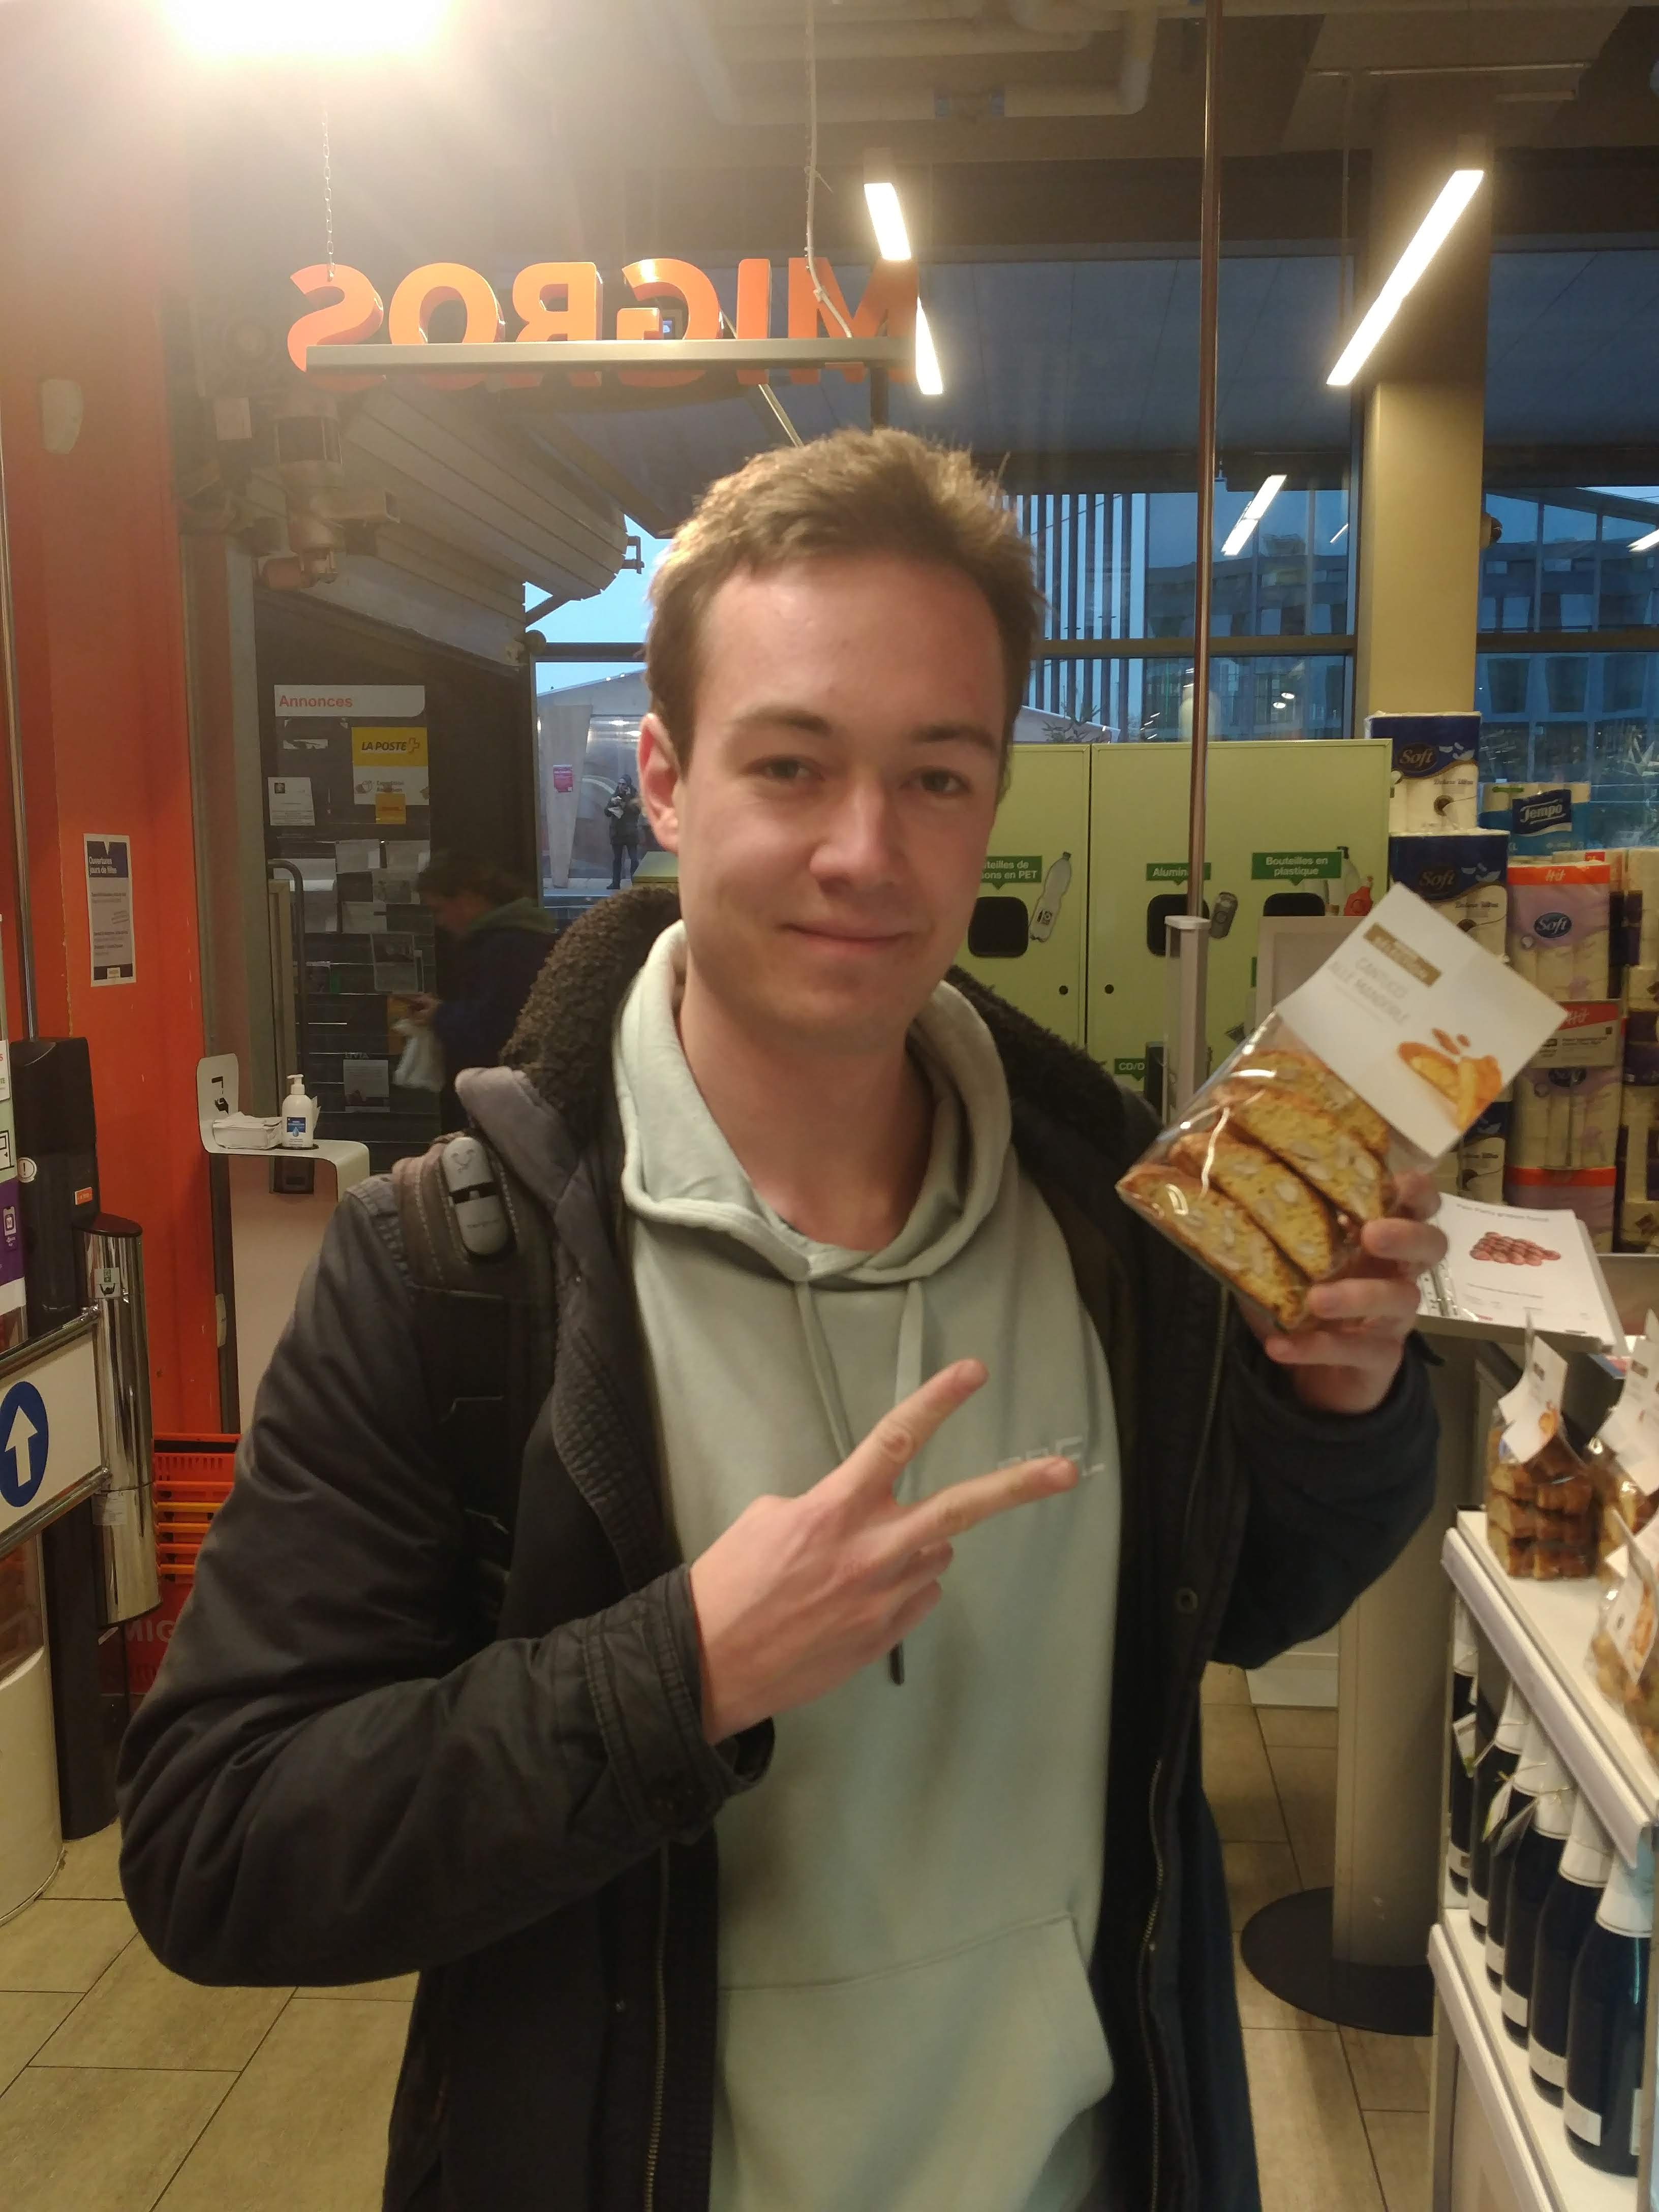
\includegraphics[width=.3\textwidth]{../_00FINAL_PROJECT/src/mandelbrot_und_so.jpg}
    \end{figure}
\end{frame}


\section{Pong}
\begin{frame}
    \sectionpage
\end{frame}

\begin{frame}
    \frametitle{Pong}
    \framesubtitle{Controll architecture}
    Elements used:
    \begin{itemize}
        \item Counters for X and Y of ball
        \item Counter for X of plate
        \item Control signals for game state
    \end{itemize}



\end{frame}


\end{document}